\documentclass[
]{jss}

\usepackage[utf8]{inputenc}

\providecommand{\tightlist}{%
  \setlength{\itemsep}{0pt}\setlength{\parskip}{0pt}}

\author{
Sahir Bhatnagar *\\McGill University \And Maxime Turgeon *\\University of Manitoba \AND Jesse Islam\\McGill University \And James Hanley\\McGill University \And Olli Saarela\\University of Toronto
}
\title{\pkg{casebase}: An Alternative Framework For Survival Analysis}

\Plainauthor{Sahir Bhatnagar *, Maxime Turgeon *, Jesse Islam, James Hanley, Olli Saarela}
\Plaintitle{casebase: An Alternative Framework For Survival Analysis}
\Shorttitle{\pkg{casebase}: An Alternative Framework For Survival Analysis}

\Abstract{
The abstract of the article. * joint co-authors
}

\Keywords{keywords, not capitalized, \proglang{Java}}
\Plainkeywords{keywords, not capitalized, Java}

%% publication information
%% \Volume{50}
%% \Issue{9}
%% \Month{June}
%% \Year{2012}
%% \Submitdate{}
%% \Acceptdate{2012-06-04}

\Address{
    Sahir Bhatnagar *\\
  McGill University\\
  1020 Pine Avenue West Montreal, QC, Canada H3A 1A2\\
  E-mail: \email{sahir.bhatnagar@mail.mcgill.ca}\\
  URL: \url{http://sahirbhatnagar.com/}\\~\\
      Maxime Turgeon *\\
  University of Manitoba\\
  186 Dysart Road Winnipeg, MB, Canada R3T 2N2\\
  E-mail: \email{max.turgeon@umanitoba.ca}\\
  URL: \url{https://maxturgeon.ca/}\\~\\
      Jesse Islam\\
  McGill University\\
  1020 Pine Avenue West Montreal, QC, Canada H3A 1A2\\
  E-mail: \email{jesse.islam@mail.mcgill.ca}\\
  
      James Hanley\\
  McGill University\\
  1020 Pine Avenue West Montreal, QC, Canada H3A 1A2\\
  E-mail: \email{james.hanley@mcgill.ca}\\
  URL: \url{http://www.medicine.mcgill.ca/epidemiology/hanley/}\\~\\
      Olli Saarela\\
  University of Toronto\\
  Dalla Lana School of Public Health, 155 College Street, 6th floor,
  Toronto, Ontario M5T 3M7, Canada\\
  E-mail: \email{olli.saarela@utoronto.ca}\\
  URL: \url{http://individual.utoronto.ca/osaarela/}\\~\\
  }

% Pandoc header

\usepackage{amsmath} \usepackage{longtable} \usepackage{graphicx} \usepackage{tabularx} \usepackage{float} \usepackage{booktabs} \usepackage{makecell} \DeclareUnicodeCharacter{2500}{-}

\begin{document}

\hypertarget{introduction}{%
\section{Introduction}\label{introduction}}

The purpose of the \pkg{casebase} package is to provide practitioners
with an easy-to-use software tool to predict the risk (or cumulative
incidence (CI)) of an event, for a particular patient. The following
points should be noted:

\begin{enumerate}
\def\labelenumi{\arabic{enumi}.}
\tightlist
\item
  hazard ratios
\item
  If, however, the absolute risks are of interest, they have to be
  recovered using the semi-parametric Breslow estimator
\item
  Alternative approaches for fitting flexible hazard models for
  estimating absolute risks, not requiring this two-step approach? Yes!
  \citep{hanley2009fitting}
\end{enumerate}

\citep{hanley2009fitting} propose a fully parametric hazard model that
can be fit via logistic regression. From the fitted hazard function,
cumulative incidence and, thus, risk functions of time, treatment and
profile can be easily derived.

\hypertarget{theoretical-details}{%
\section{Theoretical details}\label{theoretical-details}}

As discussed in Hanley \& Miettinen \citeyearpar{hanley2009fitting}, the
key idea behind case-base sampling is to discretize the study base into
an infinite amount of \emph{person moments}. These person moments are
indexed by both an individual in the study and a time point, and
therefore each person moment has a covariate profile, an exposure status
and an outcome status attached to it. We note that there is only a
finite number of person moments associated with the event of interest
(what Hanley \& Miettinen call the \emph{case series}). The case-base
sampling refers to the sampling from the base of a representative finite
sample called the \emph{base series}.

As shown by Saarela \& Arjas \citeyearpar{saarela2015non} (and further
expanded in Saarela \citeyearpar{saarela2016case}), writing the
likelihood arising from this data-generating mechanism using the
framework of non-homogeneous Poisson processes, we eventually reach an
expression where each person-moment's contribution is of the form
\[\frac{h(t)^{dN(t)}}{\rho(t) + h(t)},\] where \(N(t)\) is the counting
process associated with the event of interest, \(h(t)\) is the
corresponding hazard function, and \(\rho(t)\) is the hazard function
for the Poisson process associated with case-base sampling. This
parametric form suggests that we can readily estimate log-hazards of the
form \(\log(h(t)) = g(t; X)\) using logistic regression, where each
observation corresponds to a person moment, the function \(g(t; X)\) is
linear in a finite number of parameters, and where we treat
\(-\log(\rho(t))\) as an offset.

In Hanley \& Miettinen \citeyearpar{hanley2009fitting}, the authors
suggest performing case-base sampling \emph{uniformly}, i.e.~to sample
the base series uniformly from the study base. In terms of Poisson
processes, this sampling strategy corresponds essentially to a
time-homogeneous Poisson process with intensity equal to \(b/B\), where
\(b\) is the number of sampled observations in the base series, and
\(B\) is the total population-time for the study base. More complex
examples are also available; see for example Saarela \& Arjas
\citeyearpar{saarela2015non}, where the probabilities of the sampling
mechanism are proportional to the cardiovascular disease event rate
given by the Framingham score.

The \texttt{casebase} package fits the family of hazard functions of the
form

\[ h(t;X) = \exp[g(t;X)] \] where \(t\) denotes time and \(X\), the
individual's covariate profile. Different functions of \(t\) lead to
different parametric hazard models. The simplest of these models is the
one-parameter exponential distribution which is obtained by taking the
hazard function to be constant over the range of \(t\).

\[ h(t;X) = \exp(\beta_0 + \beta_1 X) \]

The instantaneous failure rate is independent of \(t\), so that the
conditional chance of failure in a time interval of specified length is
the same regardless of how long the individual has been in the study.
This is also known as the \emph{memoryless property} (Kalbfleisch and
Prentice, 2002).

The Gompertz hazard model is given by including a linear term for time:

\[ h(t;X)  = \exp(\beta_0 + \beta_1 t + \beta_2 X) \]

Use of \(\log(t)\) yields the Weibull hazard which allows for a power
dependence of the hazard on time (Kalbfleisch and Prentice, 2002):

\[ h(t;X)  = \exp(\beta_0 + \beta_1 \log(t) + \beta_2 X) \]

For competing-risk analyses with \(J\) possible events, we can show that
each person-moment's contribution of the likelihood is of the form

\[\frac{h_j(t)^{dN_j(t)}}{\rho(t) + \sum_{j=1}^Jh_j(t)},\]

where \(N_j(t)\) is the counting process associated with the event of
type \(j\) and \(h_j(t)\) is the corresponding hazard function. As may
be expected, this functional form is similar to the terms appearing in
the likelihood function for multinomial
regression.\footnote{Specifically, it corresponds to the following parametrization: \begin{align*} \log\left(\frac{P(Y=j \mid X)}{P(Y = J \mid X)}\right) = X^T\beta_j, \qquad j = 1,\ldots, J-1\end{align*}}

\hypertarget{existing-packages}{%
\section{Existing packages}\label{existing-packages}}

Survival analysis is an important branch of applied statistics and
epidemiology. Accordingly, there is a vast ecosystem of \code{R}
packages implementing different methods. In this section, we describe
how the functionalities of \pkg{casebase} compare to these packages.

At the time of writing, a cursory examination of CRAN's task view on
survival analysis reveals that there are over 250 packages related to
survival analysis \citeyearpar{survTaskView}. For the purposes of this
article, we restricted our description to packages that implement at
least one of the following features: parametric modeling,
non-proportional hazard models, competing risk analysis, penalized
estimation, and cumulative incidence curve estimation. By searching for
appropriate keywords in the \code{DESCRIPTION} file of these packages,
we found 60 relevant packages. These 60 packages were then manually
examined to determine which ones are comparable to \pkg{casebase}. In
particular, we excluded packages that were focused on a different set of
problems, such as frailty and multi-state models. The remaining 14
packages appear in Table \ref{tab:surv-pkgs}, along with a description
of some of the functionalities they offer.

Several packages implement penalized estimation for the Cox model:
\pkg{glmnet} \citeyearpar{regpathcox}, \pkg{glmpath}
\citeyearpar{park_hastie}, \pkg{penalized} \citeyearpar{l1penal},
\pkg{RiskRegression} \citeyearpar{gerds_blanche}. Moreover, some
packages also include penalized estimation in the context of Cox models
with time-varying coefficients: \pkg{CoxRidge}
\citeyearpar{perperoglou}, \pkg{rstpm2} \citeyearpar{clements_liu} and
\pkg{survival} \citeyearpar{survival-package}. On the other hand,
\pkg{casebase} provides penalized estimation in the context of
parametric hazards. To our knowledge, this is the only package to offer
this functionality.
\textcolor{red}{Is this true? Because it seems to be a logical conclusion from your paragraph.}

Parametric survival models are implemented in a handful of packages:
\pkg{CFC} \citeyearpar{sharabiani_mahani_2019}, \pkg{flexsurv}
\citeyearpar{flexsurv}, \pkg{SmoothHazard} \citeyearpar{smoothHazard},
\pkg{rsptm2} \citeyearpar{clements_liu}, \pkg{mets}
\citeyearpar{scheike2014estimating}, and \pkg{survival}. The types of
models they allow vary for each package. For example, \pkg{SmoothHazard}
is limited to Weibull distributions \citeyearpar{smoothHazard}, whereas
both \pkg{flexsurv} and \pkg{survival} allow users to supply any
distribution of their choice. Also, \pkg{flexsurv}, \pkg{smoothhazard},
\pkg{mets} and \pkg{rstpm2} also have the ability to model the effect of
time using splines, which allows flexible modeling of the hazard
function. Moreover, \pkg{flexsurv} has the ability to estimate both
scale and shape parameters for a variety of parametric families (see
Table \ref{tab:dists}). As discussed above, \pkg{casebase} can model any
parametric family whose log-hazard can be expressed as a linear model of
covariates (including time). Therefore, our package allows the user to
model the effect of time using splines, and through interaction terms
involving covariates and time, it also allows user to fit time-varying
coefficient models. However, we do not explicitly model any shape
parameter, unlike \pkg{flexsurv}.

Of the methods mentioned so far, only \pkg{CFC}, \pkg{flexsurv},
\pkg{mets} and \pkg{survival} contain implementations for competing
risks. The differentiating factor between these packages and
\pkg{casebase} is that \pkg{casebase} handles competing risks through
multiple logistic regression.
\textcolor{red}{There's a literature review of packages for competing-risk analysis in the paper for \pkg{CFC}. Could you incorporate some of their discussion, with proper citations? The biggest omission right now is \pkg{cmprsk}, which we actually use below.}

Finally, several packages include functions to estimate the cumulative
incidence function. The corresponding methods generally fall into two
categories: transformation of the estimated hazard function, and
semi-parametric estimation of the baseline hazard. The first category
broadly corresponds to parametric survival models, where the full hazard
is explictly modeled. Using this estimate, the survival function and the
cumulative incidence function can be obtained using their functional
relationships (see Equations \ref{eqn:surv} and \ref{eqn:CI} below).
Packages including this functionality include \pkg{CFC}, \pkg{Flexsurv},
\pkg{mets}, and \pkg{survival}. Our package \pkg{casebase} also follows
this approach for both single-event and competing-event analyses. The
second category outlined above broadly corresponds to Cox models. These
models do not model the full hazard function, and therefore the baseline
hazard needs to be estimated separately in order to estimate the
survival function. This is achieved using semi-parametric estimators
(e.g.~Breslow's estimator). Packages that implement this approach
include \pkg{RiskRegression}, \pkg{rstpm2}, and \pkg{survival}. As
mentioned in the introduction, a key distinguishing factor between these
two approaches is that the first category leads to smooth estimates of
the cumulative incidence function, whereas the second category produces
estimates in the form of step-wise functions. This was one of the main
motivations for introducting case-base sampling in survival analysis.

\begin{table}[ht]
\centering
\resizebox{\textwidth}{!}{%
\begin{tabular}{ccccccccc}
\hline
\textbf{Package}        & \vtop{\hbox{\strut \textbf{Competing}}\hbox{\strut \textbf{risks}}}  & \textbf{Non-proportional} & \textbf{Penalization} & \textbf{Splines} & \textbf{Parametric} & \textbf{Semi-parametric} & \vtop{\hbox{\strut \textbf{Interval/left}}\hbox{\strut \textbf{censoring}}} & \vtop{\hbox{\strut \textbf{Absolute}}\hbox{\strut \textbf{risk}}}           \\
\hline
\textbf{casebasee} \cite{hanley2009fitting}       & x                        & x                         & x                     & x                & x                   &                          &                                  & x                                \\
\textbf{CFC} \cite{sharabiani_mahani_2019}            & x                        & x                         &                       &                  & x                   &                          &                                  & x                                \\
\textbf{coxRidge} \cite{perperoglou}       &                          & x                         & x                     &                  &                     & x                        &                                  &                                  \\
\textbf{crrp} \cite{fu}           & x                        &                           & x                     &                  &                     &                          &                                  &                                  \\
\textbf{fastcox} \cite{yi_zou}        &                          &                           & x                     &                  &                     & x                        &                                  &                                  \\
\textbf{Flexrsurv} \cite{flexrsurv}      &                          & x                         &                       & x                & x                   &                          &                                  & x               \\
\textbf{Flexsurv} \cite{flexsurv}       & x                        & x                         &                       & x                & x                   &                          &                                  & x               \\
\textbf{glmnet} \cite{regpathcox}         &                          &                           & x                     &                  &                     & x                        &                                  &                                  \\
\textbf{glmpath} \cite{park_hastie}       &                          &                           & x                     &                  &                     & x                        &                                  &                                  \\
\textbf{mets} \cite{scheike2014estimating}           & x                        &                           &                       & x                &                     & x                        &                                  & x                                \\
\textbf{penalized} \cite{goeman_meijer2019}      &                          &                           & x                     &                  &                     & x                        &                                  &                                  \\
\textbf{RiskRegression} \cite{gerds_blanche} &                          &                           & x                     &                  &                     & x                        &                                  & x                                \\
\textbf{Rstpm2} \cite{clements_liu}         &                          & x                         & x                     & x                & x                   & x                        & x                                & x                         \\
\textbf{SmoothHazard} \cite{smoothHazard}   &                          & x                         &                       & x                & x                   &                          & x                            &                                      \\
\textbf{Survival} \cite{survival-package}       & x                        & x                         &                       &                  & x                   & x                        & x                                & x                               
\end{tabular}%
}
\caption{Different features of interest in various survival packages.}
\label{tab:surv-pkgs}
\end{table}

\begin{table}
  \begin{tabular}{p{1.8in}lll}
\hline
    &  Parameters &  Density \proglang{R} function & \code{dist}\\
    & {\footnotesize{(location in \code{\color{red}{red}})}} & & \\
\hline
    Exponential & \code{\color{red}{rate}}             & \code{dexp}   & \code{"exp"} \\
    Weibull (accelerated failure time)     & \code{shape, {\color{red}{scale}}}     & \code{dweibull} & \code{"weibull"} \\
    Weibull (proportional hazards)     & \code{shape, {\color{red}{scale}}}     & \code{dweibullPH} & \code{"weibullPH"} \\
    Gamma       & \code{shape, \color{red}{rate}}      & \code{dgamma} & \code{"gamma"}\\
    Log-normal  & \code{{\color{red}{meanlog}}, sdlog}   & \code{dlnorm} & \code{"lnorm"}\\
    Gompertz    & \code{shape, {\color{red}{rate}}}      & \code{dgompertz} & \code{"gompertz"} \\
    Log-logistic & \code{shape, {\color{red}{scale}}}   & \code{dllogis} & \code{"llogis"}\\
    Generalized gamma (Prentice 1975)   & \code{{\color{red}{mu}}, sigma, Q} & \code{dgengamma} & \code{"gengamma"} \\
    Generalized gamma (Stacy 1962)& \code{shape, {\color{red}{scale}}, k} & \code{dgengamma.orig} & \code{"gengamma.orig"} \\
    Generalized F     (stable)    & \code{{\color{red}{mu}}, sigma, Q, P} & \code{dgenf} & \code{"genf"} \\
    Generalized F     (original)  & \code{{\color{red}{mu}}, sigma, s1, s2} & \code{dgenf.orig} & \code{"genf.orig"} \\
\hline
  \end{tabular}
  \caption{Built-in parametric survival distributions in \pkg{flexsurv}.}
  \label{tab:dists}
\end{table}

\hypertarget{implementation-details}{%
\section{Implementation details}\label{implementation-details}}

The functions in the casebase package can be divided into two
categories: 1) data visualization, in the form of population-time plots;
and 2) parametric modeling. We explicitly aimed at being compatible with
both \code{data.frame}s and \code{data.table}s. This is evident in some
of the coding choices we made, and it is also reflected in our unit
tests.

\hypertarget{population-time-plots}{%
\subsection{Population-time plots}\label{population-time-plots}}

\hypertarget{parametric-modeling}{%
\subsection{Parametric modeling}\label{parametric-modeling}}

The parametric modeling step was separated into three parts:

\begin{enumerate}
\def\labelenumi{\arabic{enumi}.}
\tightlist
\item
  case-base sampling;
\item
  estimation of the smooth hazard function;
\item
  calculation of the risk function.
\end{enumerate}

By separating the sampling and estimation functions, we allowed the
possibility of users implementing more complex sampling scheme, as
described in Saarela \citeyearpar{saarela2016case}.

The sampling scheme selected for \code{sampleCaseBase} was described in
Hanley and Miettinen \citeyearpar{hanley2009fitting}: we first sample
along the ``person'' axis, proportional to each individual's total
follow-up time, and then we sample a moment uniformly over their
follow-up time. This sampling scheme is equivalent to the following
picture: imagine representing the total follow-up time of all
individuals in the study along a single dimension, where the follow-up
time of the next individual would start exactly when the follow-up time
of the previous individual ends. Then the base series could be sampled
uniformly from this one-dimensional representation of the overall
follow-up time. In any case, the output is a dataset of the same class
as the input, where each row corresponds to a person-moment. The
covariate profile for each such person-moment is retained, and an offset
term is added to the dataset. This output could then be used to fit a
smooth hazard function, or for visualization of the base series.

The fitting function \code{fitSmoothHazard} starts by looking at the
class of the dataset: if it was generated from \code{sampleCaseBase}, it
automatically inherited the class \code{cbData}. If the dataset supplied
to \code{fitSmoothHazard} does not inherit from \code{cbData}, then the
fitting function starts by calling \code{sampleCaseBase} to generate the
base series. In other words, the occasional user can bypass
\code{sampleCaseBase} altogether and only worry about the fitting
function \code{fitSmoothHazard}.

The fitting function retains the familiar formula interface of
\code{glm}. The left-hand side of the formula should be the name of the
column corresponding to the event type. The right-hand side can be any
combination of the covariates, along with an explicit functional form
for the time variable. Note that non-proportional hazard models can be
achieved at this stage by adding an interaction term involving time. The
offset term does not need to be specified by the user, as it is
automatically added to the formula.

To fit the hazard function, we provide several approaches that are
available via the \code{family} parameter. These approaches are:

\begin{itemize}
\tightlist
\item
  \code{glm}: This is the familiar logistic regression.
\item
  \code{glmnet}: This option allows for variable selection using Lasso
  or elastic-net. This functionality is provided through the
  \code{glmnet} package \citep{friedman2010jss}.
\item
  \code{gam}: This option provides support for \emph{Generalized
  Additive Models} via the \code{gam} package
  \citep{hastie1987generalized}.
\item
  \code{gbm}: This option provides support for \emph{Gradient Boosted
  Trees} via the \code{gbm} package. This feature is still experimental.
\end{itemize}

In the case of multiple events, the hazard is fitted via multinomial
regression as performed by the \pkg{VGAM} package. This package was
selected for its ability to fit multinomial regression models with an
offset.

Once a model-fit object has been returned by \code{fitSmoothHazard}, all
the familiar summary and diagnostic functions are available:
\code{print}, \code{summary}, \code{predict}, \code{plot}, etc. Our
package provides one more functionality: it computes risk functions from
the model fit. For the case of a single event, it uses the familiar
identity \begin{equation}\label{eqn:surv}
S(t) = \exp\left(-\int_0^t h(u;X) du\right).
\end{equation} The integral is computed using either the
\code{stats::integrate} function or Monte-Carlo integration. The risk
function (or cumulative incidence function) is then defined as
\begin{equation}\label{eqn:CI}
CI(t) = 1 - S(t).
\end{equation}

For the case of a competing-event analysis, the event-specific risk is
computed using the following procedure: first, we compute the overall
survival function (i.e.~for all event types):

\[ S(t) = \exp\left(-\int_0^t H(u;X) du\right),\qquad H(t;X) = \sum_{j=1}^J h_j(t;X).\]
From this, we can derive the event-specific subdensities:

\[ f_j(t) = h_j(t)S(t).\]

Finally, by integrating these subdensities, we obtain the event-specific
cumulative incidence functions:

\[ CI_j(t) = \int_0^t f_j(u)du.\]

We created \code{absoluteRisk} as an \code{S3} generic, with methods for
the different types of outputs of \code{fitSmoothHazard}. The method
dispatch system of \proglang{R} then takes care of matching the correct
output to the correct methodology for calculating the cumulative
incidence function, without the user's intervention.

In the following sections, we illustrate these functionalities in the
context of three case studies.

\hypertarget{case-study-1european-randomized-study-of-prostate-cancer-screening}{%
\section{Case study 1--European Randomized Study of Prostate Cancer
Screening}\label{case-study-1european-randomized-study-of-prostate-cancer-screening}}

For the first case study, we will use of the European Randomized Study
of Prostate Cancer Screening data. This dataset is available through the
\pkg{casebase} package:

\begin{CodeChunk}

\begin{CodeInput}
R> data(ERSPC)
R> ERSPC$ScrArm <- factor(ERSPC$ScrArm, 
R>                        levels = c(0, 1), 
R>                        labels = c("Control group", "Screening group"))
\end{CodeInput}
\end{CodeChunk}

The results of this study were published by
\citep{schroder2009screening}, and the dataset itself was obtained using
the approach described in \citep{liu2014recovering}.

Population time plots can be extremely informative graphical displays of
survival data. They should be the first step in an exploratory data
analysis. We facilitate this task in the \pkg{casebase} package using
the \code{popTime} function. We first create the necessary dataset for
producing the population time plots, and we can generate the plot by
using the corresponding \code{plot} method:

\begin{CodeChunk}

\begin{CodeInput}
R> pt_object <- casebase::popTime(ERSPC, event = "DeadOfPrCa")
R> plot(pt_object)
\end{CodeInput}
\end{CodeChunk}

We can also create exposure stratified plots by specifying the
\code{exposure} argument in the \code{popTime} function:

\begin{CodeChunk}

\begin{CodeInput}
R> pt_object_strat <- casebase::popTime(ERSPC, 
R>                                      event = "DeadOfPrCa", 
R>                                      exposure = "ScrArm")
R> plot(pt_object_strat)
\end{CodeInput}
\end{CodeChunk}

We can also plot them side-by-side using the \code{ncol} argument:

\begin{CodeChunk}

\begin{CodeInput}
R> plot(pt_object_strat, ncol = 2)
\end{CodeInput}
\end{CodeChunk}

ADD PARAGRAPH ABOUT WHAT WE CAN CONCLUDE FROM THESE GRAPHS.

Next, we investigate the differences between the control and the
screening arms. A common choice for this type of analysis is to use a
Cox regression model and estimate the hazard ratio for the screening
group (relative to the control group). In \proglang{R}, it can be done
as follows:

\begin{CodeChunk}

\begin{CodeInput}
R> cox_model <- survival::coxph(Surv(Follow.Up.Time, DeadOfPrCa) ~ ScrArm, 
R>                              data = ERSPC)
R> summary(cox_model)
\end{CodeInput}
\end{CodeChunk}

We can also plot the cumulative incidence function (CIF) for each group.
However, this involves estimating the baseline hazard, which Cox
regression treated as a nuisance parameter.

\begin{CodeChunk}

\begin{CodeInput}
R> new_data <- data.frame(ScrArm = c("Control group", "Screening group"),
R>                        ignore = 99)
R> 
R> plot(survfit(cox_model, newdata = new_data),
R>      xlab = "Years since Randomization", 
R>      ylab = "Cumulative Incidence (%)", 
R>      fun = "event",
R>      xlim = c(0,15), conf.int = FALSE, col = c("red","blue"), 
R>      main = sprintf("Estimated Cumulative Incidence (risk) of Death from Prostate 
R>                     Cancer Screening group Hazard Ratio: %.2g (%.2g, %.2g)",
R>                     exp(coef(cox_model)), 
R>                     exp(confint(cox_model))[1], 
R>                     exp(confint(cox_model))[2]),
R>      ylim = c(0, 2), yscale = 100)
R> legend("topleft", 
R>        legend = c("Control group", "Screening group"), 
R>        col = c("red","blue"),
R>        lty = c(1, 1), 
R>        bg = "gray90")
\end{CodeInput}
\end{CodeChunk}

Next, we show how case-base sampling can be used to carry out a similar
analysis. We fit several models that differ in how we choose to model
time.

First, we will fit an exponential model. Recall that this corresponds to
excluding time from the linear predictor.

\begin{CodeChunk}

\begin{CodeInput}
R> casebase_exponential <- casebase::fitSmoothHazard(DeadOfPrCa ~ ScrArm, 
R>                                                   data = ERSPC, 
R>                                                   ratio = 100)
R> 
R> summary(casebase_exponential)
R> exp(coef(casebase_exponential)[2])
R> exp(confint(casebase_exponential)[2,])
\end{CodeInput}
\end{CodeChunk}

We can then use the \code{absoluteRisk} function to get an estimate of
the cumulative incidence curve for a specific covariate profile. In the
plot below, we overlay the estimated CIF from the exponential model on
the Cox model CIF:

\begin{CodeChunk}

\begin{CodeInput}
R> smooth_risk_exp <- casebase::absoluteRisk(object = casebase_exponential, 
R>                                           time = seq(0,15,0.1), 
R>                                           newdata = new_data)
R> 
R> plot(survfit(cox_model, newdata = new_data),
R>      xlab = "Years since Randomization", 
R>      ylab = "Cumulative Incidence (%)", 
R>      fun = "event",
R>      xlim = c(0,15), conf.int = FALSE, col = c("red","blue"), 
R>      main = sprintf("Estimated Cumulative Incidence (risk) of Death from Prostate 
R>                     Cancer Screening group Hazard Ratio: %.2g (%.2g, %.2g)",
R>                     exp(coef(cox_model)), 
R>                     exp(confint(cox_model))[1], 
R>                     exp(confint(cox_model))[2]),
R>      ylim = c(0, 2), yscale = 100)
R> lines(smooth_risk_exp[,1], smooth_risk_exp[,2], col = "red", lty = 2)
R> lines(smooth_risk_exp[,1], smooth_risk_exp[,3], col = "blue", lty = 2)
R> 
R> 
R> legend("topleft", 
R>        legend = c("Control group (Cox)","Control group (Casebase)",
R>                   "Screening group (Cox)", "Screening group (Casebase)"), 
R>        col = c("red","red", "blue","blue"),
R>        lty = c(1, 2, 1, 2), 
R>        bg = "gray90")
\end{CodeInput}
\end{CodeChunk}

As we can see, the exponential model gives us an estimate of the hazard
ratio that is similar to the one obtained using Cox regression. However,
the CIF estimates are quite different. Based on what we observed in the
population time plot, where more events are observed later on in time,
we do not expect a constant hazard would be a good description for this
data. In other words, this poor fit for the exponential hazard is
expected. A constant hazard model would overestimate the cumulative
incidence earlier on in time, and underestimate it later on; this is
what we see on the cumulative incidence plot. This example demonstrates
the benefits of population time plots as an exploratory analysis tool.

For the next model, we include time as a linear term. Recall that this
corresponds to a Weibull model.

\begin{CodeChunk}

\begin{CodeInput}
R> casebase_time <- fitSmoothHazard(DeadOfPrCa ~ Follow.Up.Time + ScrArm, 
R>                                  data = ERSPC, 
R>                                  ratio = 100)
R> 
R> summary(casebase_time)
R> exp(coef(casebase_time))
R> exp(confint(casebase_time))
\end{CodeInput}
\end{CodeChunk}

Again, the estimate of the hazard ratio is similar to that obtained from
Cox regression. We then look at the estimate of the CIF:

\begin{CodeChunk}

\begin{CodeInput}
R> smooth_risk_time <- casebase::absoluteRisk(object = casebase_time, 
R>                                           time = seq(0,15,0.1), 
R>                                           newdata = new_data)
R> 
R> plot(survfit(cox_model, newdata = new_data),
R>      xlab = "Years since Randomization", 
R>      ylab = "Cumulative Incidence (%)", 
R>      fun = "event",
R>      xlim = c(0,15), conf.int = FALSE, col = c("red","blue"), 
R>      main = sprintf("Estimated Cumulative Incidence (risk) of Death from Prostate 
R>                     Cancer Screening group Hazard Ratio: %.2g (%.2g, %.2g)",
R>                     exp(coef(cox_model)), 
R>                     exp(confint(cox_model))[1], 
R>                     exp(confint(cox_model))[2]),
R>      ylim = c(0, 2), yscale = 100)
R> lines(smooth_risk_time[,1], smooth_risk_time[,2], col = "red", lty = 2)
R> lines(smooth_risk_time[,1], smooth_risk_time[,3], col = "blue", lty = 2)
R> 
R> legend("topleft", 
R>        legend = c("Control group (Cox)","Control group (Casebase)",
R>                   "Screening group (Cox)", "Screening group (Casebase)"), 
R>        col = c("red","red", "blue","blue"),
R>        lty = c(1, 2, 1, 2), 
R>        bg = "gray90")
\end{CodeInput}
\end{CodeChunk}

We see that the Weibull model leads to a better fit of the CIF than the
Exponential model, when compared with the semi-parametric approach.

Finally, we can model the hazard as a smooth function of time using the
\code{splines} package:

\begin{CodeChunk}

\begin{CodeInput}
R> casebase_splines <- fitSmoothHazard(DeadOfPrCa ~ bs(Follow.Up.Time) + ScrArm, 
R>                                     data = ERSPC, 
R>                                     ratio = 100)
R> 
R> summary(casebase_splines)
R> exp(coef(casebase_splines))
R> exp(confint(casebase_splines))
\end{CodeInput}
\end{CodeChunk}

Once again, we can see that the estimate of the hazard ratio is similar
to that from the Cox regression. We then look at the estimate of the
CIF:

\begin{CodeChunk}

\begin{CodeInput}
R> smooth_risk_splines <- absoluteRisk(object = casebase_splines, 
R>                                     time = seq(0,15,0.1), 
R>                                     newdata = new_data)
R> 
R> plot(survfit(cox_model, newdata = new_data),
R>      xlab = "Years since Randomization", 
R>      ylab = "Cumulative Incidence (%)", 
R>      fun = "event",
R>      xlim = c(0,15), conf.int = FALSE, col = c("red","blue"), 
R>      main = sprintf("Estimated Cumulative Incidence (risk) of Death from Prostate 
R>                     Cancer Screening group Hazard Ratio: %.2g (%.2g, %.2g)",
R>                     exp(coef(cox_model)), 
R>                     exp(confint(cox_model))[1], 
R>                     exp(confint(cox_model))[2]),
R>      ylim = c(0, 2), yscale = 100)
R> lines(smooth_risk_splines[,1], smooth_risk_splines[,2], col = "red", lty = 2)
R> lines(smooth_risk_splines[,1], smooth_risk_splines[,3], col = "blue", lty = 2)
R> 
R> legend("topleft", 
R>        legend = c("Control group (Cox)","Control group (Casebase)",
R>                   "Screening group (Cox)", "Screening group (Casebase)"), 
R>        col = c("red","red", "blue","blue"),
R>        lty = c(1, 2, 1, 2), 
R>        bg = "gray90")
\end{CodeInput}
\end{CodeChunk}

Qualitatively, the combination of splines and case-base sampling
produces the parametric model that most closely resembles the Cox model.
In the following table, we see that the confidence intervals are also
similar across all four models. In other words, this reinforces the idea
that, under proportional hazards, we do not need to model the full
hazard to obtain reliable estimates of the hazard ratio. Of course,
different parametric models for the hazards give rise to qualitatively
different estimates for the CIF.

As noted above, the usual asymptotic results hold for likelihood ratio
tests built using case-base sampling models. Therefore, we can easily
test the null hypothesis that the exponential model is just as good as
the larger (in terms of number of parameters) splines model.

\begin{CodeChunk}

\begin{CodeInput}
R> anova(casebase_exponential, casebase_splines, test = "LRT")
\end{CodeInput}
\end{CodeChunk}

As expected, we see that splines model provides a better fit. Similarly,
we can compare the AIC for all three case-base models:

\begin{CodeChunk}

\begin{CodeInput}
R> c("Exp." = AIC(casebase_exponential),
R>   "Weib." = AIC(casebase_time),
R>   "Splines" = AIC(casebase_splines))
\end{CodeInput}
\end{CodeChunk}

Once again, we have evidence that the splines model provides the best
fit.

With this first case study, we saw how population-time plots can provide
a useful summary of the incidence for our event of interests. In
particular, we saw how it can provide evidence against an exponential
hazard model. We then explored how different parametric models can
provide different estimates of the CIF, even though they all give
similar estimates for the hazard ratios.

\hypertarget{case-study-2bone-marrow-transplant}{%
\section{Case study 2--Bone-marrow
transplant}\label{case-study-2bone-marrow-transplant}}

In the next case study, we show how case-base sampling can also be used
in the context of a competing risk analysis. For illustrative purposes,
we will use the same data that was used in Scrucca \emph{et al}
\citeyearpar{scrucca2010regression}. The data was downloaded from the
first author's website, and it is also available as part of the
\pkg{casebase} package.

\begin{CodeChunk}

\begin{CodeInput}
R> library(casebase)
R> data(bmtcrr)
\end{CodeInput}
\end{CodeChunk}

The data contains information on 177 patients who received a stem-cell
transplant for acute leukemia. The event of interest is relapse, but
other competing causes (e.g.~transplant-related death) were also
recorded. Several covariates were captured at baseline: sex, disease
type (acute lymphoblastic or myeloblastic leukemia, abbreviated as ALL
and AML, respectively), disease phase at transplant (Relapse, CR1, CR2,
CR3), source of stem cells (bone marrow and peripheral blood, coded as
BM+PB, or only peripheral blood, coded as PB), and age. A summary of
these baseline characteristics appear in Table \ref{tab:table1bmtcrr}.
We note that the statistical summaries were generated differently for
different variable types: for continuous variables, we gave the range,
followed by the mean and standard deviation; for categorical variables,
we gave the counts for each category.

First, we can look at a population-time plot to visualize the incidence
density of both relapse and the competing events. In Figure
\ref{fig:compPop}, failure times are highlighted on the plot using red
points for the event of interest (panel A) and blue dots for competing
events (panel B). In both panels, we see evidence of a non-constant
hazard function: the density of points is larger at the beginning of
follow-up than at the end.

Our main objective is to compute the absolute risk of relapse for a
given set of covariates. First, we fit a smooth hazard to the data using
a linear term for time:

\begin{CodeChunk}

\begin{CodeInput}
R> model_cb <- fitSmoothHazard(
R>     Status ~ ftime + Sex + D + Phase + Source + Age, 
R>     data = bmtcrr, 
R>     ratio = 100, 
R>     time = "ftime")
\end{CodeInput}
\end{CodeChunk}

We will compare our hazard ratio estimates to that obtained from a Cox
regression. To do so, we need to treat the competing event as censoring.

\begin{CodeChunk}

\begin{CodeInput}
R> library(survival)
R> # Treat competing event as censoring
R> model_cox <- coxph(Surv(ftime, Status == 1) ~ Sex + D + Phase + Source + Age,
R>                    data = bmtcrr)
\end{CodeInput}
\end{CodeChunk}

From the fit object, we can extract both the hazard ratios and their
corresponding confidence intervals. These quantities appear in Table
\ref{tab:bmtcrr-cis}. As we can see, the only significant hazard ratio
identified by case-base sampling is the one associated with the phase of
the disease at transplant. More precisely, being in relapse at
transplant is associated with a hazard ratio of 3.89 when compared to
CR1.

Given the estimate of the hazard function obtained using case-base
sampling, we can compute the absolute risk curve for a fixed covariate
profile. We perform this computation for a 35 year old woman who
received a stem-cell transplant from peripheral blood at relapse. We
compared the absolute risk curve for such a woman with acute
lymphoblastic leukemia with that for a similar woman with acute
myeloblastic leukemia. We will estimate the curve from 0 to 60 months.

\begin{CodeChunk}

\begin{CodeInput}
R> # Pick 100 equidistant points between 0 and 60 months
R> time_points <- seq(0, 60, length.out = 50)
R> 
R> # Data.frame containing risk profile
R> newdata <- data.frame("Sex" = factor(c("F", "F"), 
R>                                      levels = levels(bmtcrr[,"Sex"])),
R>                       "D" = c("ALL", "AML"), # Both diseases
R>                       "Phase" = factor(c("Relapse", "Relapse"), 
R>                                        levels = levels(bmtcrr[,"Phase"])),
R>                       "Age" = c(35, 35),
R>                       "Source" = factor(c("PB", "PB"), 
R>                                         levels = levels(bmtcrr[,"Source"])))
R> 
R> # Estimate absolute risk curve
R> risk_cb <- absoluteRisk(object = model_cb, time = time_points,
R>                         method = "numerical", newdata = newdata)
\end{CodeInput}
\end{CodeChunk}

We will compare our estimates to that obtained from a corresponding
Fine-Gray model \citep{fine1999proportional}. The Fine-Gray model is a
semiparametric model for the cause-specific \emph{subdistribution},
i.e.~the function \(f_k(t)\) such that
\[CI_k(t) =1 - \exp\left( - \int_0^t f_k(u) \textrm{d}u \right),\] where
\(CI_k(t)\) is the cause-specific cumulative indicence. The Fine-Gray
model allows to directly assess the effect of a covariate on the
subdistribution, as opposed to the hazard. For the computation, we will
use the \pkg{timereg} package \citep{timereg}.

\begin{CodeChunk}

\begin{CodeInput}
R> library(timereg)
R> model_fg <- comp.risk(Event(ftime, Status) ~ const(Sex) + const(D) + 
R>                           const(Phase) + const(Source) + const(Age), 
R>                       data = bmtcrr, cause = 1, model = "fg")
R> 
R> # Estimate absolute risk curve
R> risk_fg <- predict(model_fg, newdata, times = time_points)
\end{CodeInput}
\end{CodeChunk}

Figure \ref{fig:compAbsrisk} shows the absolute risk curves for both
case-base sampling and the Fine-Gray model. As we can see, the two
approaches agree quite well for acute myeloblastic leukemia; however,
there seems to be a difference of about 5\% between the two curves for
acute lymphoblastic leukemia. This difference does not appear to be
significant: the curve from case-base sampling is contained within a
95\% confidence band around the Fine-Gray absolute risk curve (figure
not shown).

\hypertarget{case-study-3support-data}{%
\section{Case study 3--SUPPORT Data}\label{case-study-3support-data}}

In the first two case studies, we described the basic functionalities of
the \pkg{casebase} package: creating population-time plots, fitting
parametric models for hazard functions, and estimating the corresponding
cumulative incidence curves. In the next two case studies, we explore
more advanced features.

For the third case study, we will look at regularized estimation for the
hazard function. This can be performed using a combination of case-base
sampling and regularized logistic regression. To demonstrate this
capability, we examine the Study to Understand Prognoses Preferences
Outcomes and Risks of Treatment (SUPPORT) dataset
\citep{knaus1995support}. The SUPPORT dataset tracks death for
individuals who are considered seriously ill within a hospital.
Imputation was conducted using predictive mean matching and using the
\pkg{mice} package in \proglang{R} \citep{mice}. Before imputation,
there was a total of 1000 individuals and 35 variables. After
imputation, we have 474 individuals.
\textcolor{red}{How come we lose individuals during imputation?} Of
these, 67.5\% experienced the event of interest. A description of each
variable can be found in Table \ref{tab:support1} and a breakdown of
each categorical variable in Table \ref{tab:support2}. The original data
was obtained from the website of the Department of Biostatistics at
Vanderbilt University. The imputed dataset is available as part of the
\pkg{casebase} package.

\begin{table}[ht]
\centering
\begin{tabular}{ccccc}
\hline
\textbf{Name} & \textbf{Labels}                          & \textbf{Levels} & \textbf{Storage} & \textbf{NAs} \\
\hline
age           & Age                                      &                 & double           & 0            \\
death         & Death at any time up to NDI date:31DEC94 &                 & double           & 0            \\
sex           &                                          & 2               & integer          & 0            \\
hospdead      & Death in Hospital                        &                 & double           & 0            \\
slos          & Days from Study Entry to Discharge       &                 & double           & 0            \\
d.time        & Days of Follow-Up                        &                 & double           & 0            \\
dzgroup       &                                          & 8               & integer          & 0            \\
dzclass       &                                          & 4               & integer          & 0            \\
num.co        & number of comorbidities                  &                 & double           & 0            \\
edu           & Years of Education                       &                 & double           & 202          \\
income        &                                          & 4               & integer          & 349          \\
scoma         & SUPPORT Coma Score based on Glasgow D3   &                 & double           & 0            \\
charges       & Hospital Charges                         &                 & double           & 25           \\
totcst        & Total RCC cost                           &                 & double           & 105          \\
totmcst       & Total micro-cost                         &                 & double           & 372          \\
avtisst       & Average TISS, Days 3-25                  &                 & double           & 6            \\
race          &                                          & 5               & integer          & 5            \\
meanbp        & Mean Arterial Blood Pressure Day 3       &                 & double           & 0            \\
wblc          & White Blood Cell Count Day 3             &                 & double           & 24           \\
hrt           & Heart Rate Day 3                         &                 & double           & 0            \\
resp          & Respiration Rate Day 3                   &                 & double           & 0            \\
temp          & Temperature (Celsius) Day 3              &                 & double           & 0            \\
pafi          & PaO2/(.01*FiO2) Day 3                    &                 & double           & 253          \\
alb           & Serum Albumin Day 3                      &                 & double           & 378          \\
bili          & Bilirubin Day 3                          &                 & double           & 297          \\
crea          & Serum creatinine Day 3                   &                 & double           & 3            \\
sod           & Serum sodium Day 3                       &                 & double           & 0            \\
ph            & Serum pH (arterial) Day 3                &                 & double           & 250          \\
glucose       & Glucose Day 3                            &                 & double           & 470          \\
bun           & BUN Day 3                                &                 & double           & 455          \\
urine         & Urine Output Day 3                       &                 & double           & 517          \\
adlp          & ADL Patient Day 3                        &                 & double           & 634          \\
adls          & ADL Surrogate Day 3                      &                 & double           & 310          \\
sfdm2         &                                          & 5               & integer          & 159          \\
adlsc         & Imputed ADL Calibrated to Surrogate      &                 & double           & 0           
\end{tabular}
\caption{A description of each variable in the SUPPORT dataset.}
\label{tab:support1}
\end{table}

\begin{table}[ht]
\centering
\begin{tabular}{cc}
\hline
\textbf{Variable} & \textbf{Levels}                      \\
\hline
sex      & female                                        \\
         & male                                          \\
dzgroup  & ARF/MOSF w/Sepsis                             \\
         & COPD                                          \\
         & CHF                                           \\
         & Cirrhosis                                     \\
         & Coma                                          \\
         & Colon Cancer                                  \\
         & Lung Cancer                                   \\
         & MOSF w/Malig                                  \\
dzclass  & ARF/MOSF                                      \\
         & COPD/CHF/Cirrhosis                            \\
         & Coma                                          \\
         & Cancer                                        \\
income   & under \$11k                                   \\
         & $11-$25k                                      \\
         & $25-$50k                                      \\
         & \textgreater{}\$50k                           \\
race     & white                                         \\
         & black                                         \\
         & asian                                         \\
         & other                                         \\
         & hispanic                                      \\
sfdm2    & no(M2 and SIP pres)                           \\
         & adl\textgreater{}=4 (\textgreater{}=5 if sur) \\
         & SIP\textgreater{}=30                          \\
         & Coma or Intub                                 \\
         & \textless{}2 mo. follow-up                   
\end{tabular}
\caption{A description of each level within each categorical variable in the dataset.}
\label{tab:support2}
\end{table}

As before, the first step is to visualize the incidence density. The
population-time plot for the SUPPORT data appears in Figure
\ref{fig:support-poptime}.
\textcolor{red}{This population-time plot is strange. The red dots never seem to go above 200.}

\begin{CodeChunk}

\begin{CodeInput}
R> data(support)
R> support_popTime <- popTime(support,
R+                            time = "d.time", event = "death")
R> plot(support_popTime)
\end{CodeInput}
\begin{figure}

{\centering 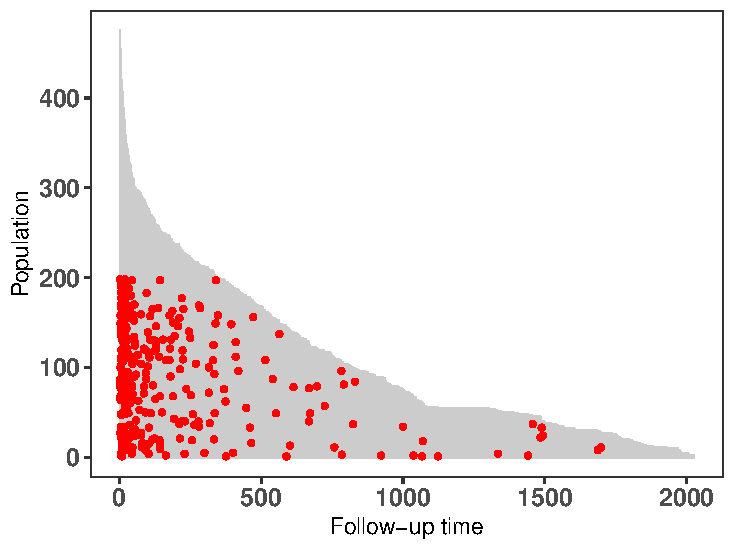
\includegraphics{../figures/support-poptime-1} 

}

\caption{\label{fig:support-poptime} Population-time plot for tje SUPPORT data.}\label{fig:support-poptime}
\end{figure}
\end{CodeChunk}

Before we proceed with the analysis, we first remove hospital death as a
covariate, as this is directly informative of death and cannot be used
as a predictor. Then we select one observation at random. We will
estimate the cumulative incidence curve for this individual. The other
observations will be used to fit the hazard function.

\begin{CodeChunk}

\begin{CodeInput}
R> support <- dplyr::select(support, -hospdead)
R> 
R> # Randomly select one observation
R> indiv <- sample(1:nrow(support), size = 1)
\end{CodeInput}
\end{CodeChunk}

Our main objective is to estimate the cumulative incidence of death for
a given covariate profile. Given the number of covariates available, we
will do this using regularized estimation. As \pkg{casebase} makes use
of the \pkg{glmnet} package, we will use the function
\code{fitsmoothhazard.fit}, which follows the syntax from \code{glmnet}.
Specifically, we input a matrix \code{y}, which contains the time and
event variables, and a matrix \code{x}, which contains all other
variables we would like to include in the model. For the SUPPORT
dataset, all factor variables were converted into dummy variables.

\begin{CodeChunk}

\begin{CodeInput}
R> # Create design matrix without the time variable
R> support_matrix <- model.matrix(death ~ . - d.time, 
R+                                data = support)
R> # Remove intercept term
R> support_matrix <- support_matrix[,colnames(support_matrix) != "(Intercept)"]
R> 
R> # Create test and train dataset
R> support_test <- support_matrix[indiv,,drop = FALSE]
R> 
R> support_train <- support_matrix[-indiv,]
R> y <- as.matrix(support[-indiv, c("death", "d.time")])
\end{CodeInput}
\end{CodeChunk}

We are now ready to estimate the hazard function. We use lasso
penalization; this is achieved by setting \code{alpha} to 1. Also, note
that the argument \code{formula_time} can be used to specify the
function form for time; in our example, we model time linearly.

\begin{CodeChunk}

\begin{CodeInput}
R> support_cb <- fitSmoothHazard.fit(support_train, y, 
R+                                   formula_time = ~ d.time, 
R+                                   family = "glmnet", 
R+                                   event = "death", time = "d.time", 
R+                                   alpha = 1, ratio = 100)
\end{CodeInput}
\end{CodeChunk}

Then, we take our model object and use the \code{absoluteRisk} function
to compute our estimate of the cumulative incidence function. Since
\code{glmnet} fitted the penalized logistic regression for a range of
penalty terms, we need to specify which one we want to use for our
prediction. We select \code{s = "lambda.1se"}, as recommended.

\begin{CodeChunk}

\begin{CodeInput}
R> time_points <- seq(1, max(support$d.time), by = 0.5)
R> support_risk <- absoluteRisk(support_cb,
R+                              time = time_points,
R+                              newdata = support_test,
R+                              s = "lambda.1se", method = "numerical")
\end{CodeInput}
\end{CodeChunk}

We will compare this curve to a regularized version of Cox regression,
and a Kaplan-Meier survival curve. Using the \pkg{glmnet} package, we
can fit the Cox regression model using regularized estimation.

\begin{CodeChunk}

\begin{CodeInput}
R> # Create survival object for glmnet
R> surv_glmnet <- survival::Surv(time = y[, "d.time"], 
R+                               event = y[, "death"])
R> 
R> support_cox <- glmnet::cv.glmnet(x = support_train, 
R+                                  y = surv_glmnet,
R+                                  family = "cox", alpha = 1)
\end{CodeInput}
\end{CodeChunk}

However, \pkg{glmnet} does not provide any functionality for estimating
the baseline hazard, and the functionalities in the \pkg{survival}
package do not work on the output from \code{cv.glmnet}. To circumvent
this issue and get an estimate of the baseline hazard, we followed the
following steps. First, we fitted a non-regularized Cox model using only
the variables selected by \pkg{glmnet}; the baseline hazard will be
estimated using this object. Then, we replaced the estimates of the
regression coefficients by the estimates from \pkg{glmnet}. Finally,
this modified \code{coxph} object is fed to the \code{survival::survfit}
function to obtain the estimated survival function.

\begin{CodeChunk}

\begin{CodeInput}
R> # Identifying selected covariates
R> nonzero_covariates_cox <- predict(support_cox, type = "nonzero", 
R+                                   s = "lambda.1se")
R> nonzero_coef_cox <- coef(support_cox, s = "lambda.1se")
R> # Creating a new dataset that only contains the covariates selected by glmnet
R> support_cox_data <- as.data.frame(cbind(y,
R+                                         support_train[, nonzero_covariates_cox$X1]))
R> # Fitting a cox model
R> support_cox <- survival::coxph(Surv(time = d.time, event = death) ~ ., 
R+                           data = support_cox_data)
R> # Replace the estimate with those obtained by glmnet
R> support_cox$coefficients <- nonzero_coef_cox@x
R> 
R> # Fitting CI curve for cox+glmnet
R> support_cox_risk <- survival::survfit(support_cox,
R+                                       newdata = as.data.frame(support_test),
R+                                       time = time_points,
R+                                       type = "breslow")
\end{CodeInput}
\end{CodeChunk}

We used the \pkg{survival} package to calculate the Kaplan-Meier
estimate of the survival function.

\begin{CodeChunk}

\begin{CodeInput}
R> km <- survival::Surv(time = support$d.time, 
R+                      event = support$death)
R> abKm <- survival::survfit(km ~ 1,
R+                           type = 'kaplan-meier')
\end{CodeInput}
\end{CodeChunk}

Now that our three cumulative incidence functions have been calculated,
we compare them all in Figure \ref{fig:abSC}. Both \pkg{glmnet} and
\pkg{casebase} have a lower estimated cumulative incidence by the end of
the study, when compared to Kaplan-Meier.
\textcolor{red}{It would be good to have an idea of why the case-base and Coxnet curves are so different. At the very least, I think we should compare the select covariates.}

\begin{CodeChunk}
\begin{figure}

{\centering 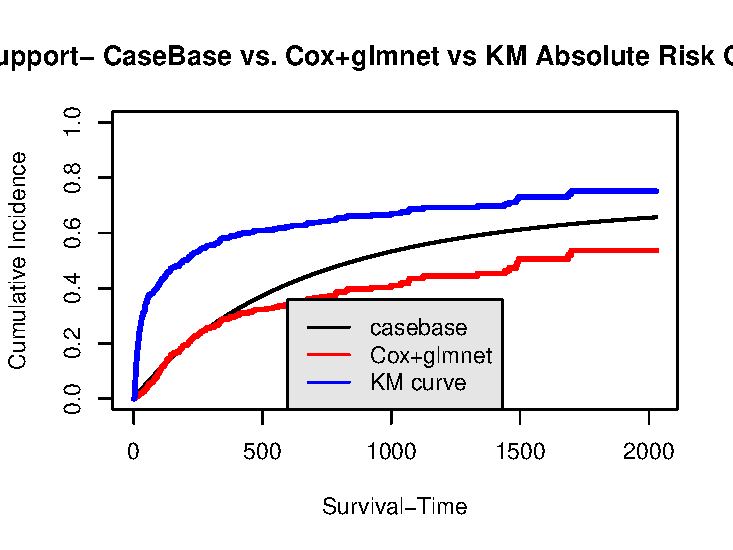
\includegraphics{../figures/abSupportComparison-1} 

}

\caption{\label{fig:abSC} Comparison of cumulative incidence curves between regularized casebase in black, regularized Cox regression in red and Kaplan-Meier in blue.}\label{fig:abSupportComparison}
\end{figure}
\end{CodeChunk}

\hypertarget{case-study-4stanford-heart-transplant-data}{%
\section{Case study 4--Stanford Heart Transplant
Data}\label{case-study-4stanford-heart-transplant-data}}

Although the previous case studies provide a broad overview of the
capabilities of \pkg{casebase}, they all have two properties in common:

\begin{itemize}
  \item All covariates are fixed, i.e. they do not change over time;
  \item The estimated hazard functions satisfy the "proportional hazard" assumption.
\end{itemize}

Case-base sampling has been used in the literature to study vaccination
safety, where the exposure period was defined as the week following
vaccination \citep{saarela2015case}. Hence, the main covariate of
interest, i.e.~exposure to the vaccine, was changing over time. In this
context, case-base sampling offers an efficient alternative to nested
case-control designs or self-matching.

The purpose of the next case study is to show how \pkg{casebase} can
also be used for survival analysis problems that do not share the
properties above. To this end, we will use the Stanford Heart Transplant
Data \citep[\citet{crowley1977covariance}]{clark1971cardiac}; we will
use the version available in the \pkg{surivival} package.

Recall the setting of this study: patients were admitted to the Stanford
program after meeting with their physician and determining that they
were unlikely to respond to other forms of treatment. After enrollment,
the program searches for a suitable donor for the patient, which can
take anywhere between a few days to almost a year. We are interested in
the effect of a heart transplant on survival; therefore, the patient is
considered exposed only after the transplant has occurred.

As before, we can look at the population-time plot for a graphical
summary of the event incidence. As we can see, most events occur early
during the follow-up period, and therefore we do not expect the hazard
to be constant.

\begin{CodeChunk}

\begin{CodeInput}
R> library(survival)
R> library(casebase)
R> 
R> stanford_popTime <- popTime(jasa, time = "futime", 
R>                             event = "fustat")
R> plot(stanford_popTime)
\end{CodeInput}
\end{CodeChunk}

Since the exposure is time-dependent, we need to manually define the
exposure variable \emph{after} case-base sampling and \emph{before}
fitting the hazard function. For this reason, we will use the
\texttt{sampleCaseBase} function directly.

\begin{CodeChunk}

\begin{CodeInput}
R> library(tidyverse)
R> library(lubridate)
R> 
R> cb_data <- sampleCaseBase(jasa, time = "futime", 
R>                           event = "fustat", ratio = 10)
\end{CodeInput}
\end{CodeChunk}

Next, we will compute the number of days from acceptance into the
program to transplant, and we use this variable to determine whether
each population-moment is exposed or not.

\begin{CodeChunk}

\begin{CodeInput}
R> # Define exposure variable
R> cb_data <- mutate(cb_data,
R>                   txtime = time_length(accept.dt %--% tx.date, 
R>                                        unit = "days"),
R>                   exposure = case_when(
R>                     is.na(txtime) ~ 0L,
R>                     txtime > futime ~ 0L,
R>                     txtime <= futime ~ 1L
R>                   ))
\end{CodeInput}
\end{CodeChunk}

Finally, we can fit the hazard using various linear predictors.

\begin{CodeChunk}

\begin{CodeInput}
R> library(splines)
R> # Fit several models
R> fit1 <- fitSmoothHazard(fustat ~ exposure,
R>                         data = cb_data, time = "futime")
R> fit2 <- fitSmoothHazard(fustat ~ exposure + futime,
R>                         data = cb_data, time = "futime")
R> fit3 <- fitSmoothHazard(fustat ~ exposure + bs(futime),
R>                         data = cb_data, time = "futime")
R> fit4 <- fitSmoothHazard(fustat ~ exposure*bs(futime),
R>                         data = cb_data, time = "futime")
\end{CodeInput}
\end{CodeChunk}

Note that the fourth model (i.e.~\texttt{fit4}) includes an interaction
term between exposure and follow-up time. In other words, this model no
longer exhibit proportional hazards. The evidence of non-proportionality
of hazards in the Stanford Heart Transplant data has been widely
discussed \citep{arjas1988graphical}.

We can then compare the goodness of fit of these four models using the
Akaike Information Criterion (AIC).

\begin{CodeChunk}

\begin{CodeInput}
R> # Compute AIC
R> c("Model1" = AIC(fit1),
R>   "Model2" = AIC(fit2),
R>   "Model3" = AIC(fit3),
R>   "Model4" = AIC(fit4))
\end{CodeInput}
\end{CodeChunk}

As we can, the best fit is the fourth model. By visualizing the hazard
functions for both exposed and unexposed individuals, we can more
clearly see how the hazards are no longer proportional.

\begin{CodeChunk}

\begin{CodeInput}
R> # Compute hazards---
R> # First, create a list of time points for both exposure status
R> hazard_data <- expand.grid(exposure = c(0, 1),
R>                            futime = seq(0, 1000,
R>                                         length.out = 100))
R> # Set the offset to zero
R> hazard_data$offset <- 0 
R> # Use predict to get the fitted values, and exponentiate to 
R> # transform to the right scale
R> hazard_data$hazard = exp(predict(fit4, newdata = hazard_data,
R>                                  type = "link"))
R> # Add labels for plots
R> hazard_data$Status = factor(hazard_data$exposure,
R>                             labels = c("NoTrans", "Trans"))
R> 
R> ggplot(hazard_data, aes(futime, hazard, colour = Status)) +
R>     geom_line() +
R>     theme_minimal() +
R>     theme(legend.position = 'top') +
R>     ylab('Hazard') + xlab('Follow-up time')
\end{CodeInput}
\end{CodeChunk}

The non-proportionality seems to be more pronounced at the beginning of
follow-up than the end. Finally, we can turn these estimate of the
hazard function into estimates of the cumulative incidence functions.

\begin{CodeChunk}

\begin{CodeInput}
R> # Compute absolute risk curves
R> newdata <- data.frame(exposure = c(0, 1))
R> absrisk <- absoluteRisk(fit4, newdata = newdata, 
R>                         time = seq(0, 1000, length.out = 100))
R> 
R> colnames(absrisk) <- c("Time", "NoTrans", "Trans")
R> 
R> # Rearrange the data
R> absrisk <- gather(as.data.frame(absrisk),
R>                   "Status", "Risk", -Time)
R>  
R> ggplot(absrisk, aes(Time, Risk, colour = Status)) +
R>   geom_line() +
R>   theme_minimal() +
R>   theme(legend.position = 'top') +
R>   expand_limits(y = 0.5) +
R>   xlab('Follow-up time') + ylab('Cum. Incidence')
\end{CodeInput}
\end{CodeChunk}

Note that we can easily adapt the code above to the situation where a
patient receives a heart transplant at a point in time of interest, for
example after 30 days.

\begin{CodeChunk}

\begin{CodeInput}
R> # Compute hazards---
R> # First, create a list of time points for both exposure status
R> one_yr_haz <- data.frame(futime = seq(0, 365,
R>                                       length.out = 100))
R> one_yr_haz <- mutate(one_yr_haz,
R>                      offset = 0,
R>                      exposure = if_else(futime < 30, 0, 1))
R> one_yr_haz$hazard = exp(predict(fit4, newdata = one_yr_haz,
R>                                 type = "link"))
R> ggplot(one_yr_haz, aes(futime, hazard)) +
R>   geom_line() +
R>   theme_minimal() +
R>   theme(legend.position = 'top') +
R>   ylab('Hazard') + xlab('Follow-up time') +
R>   geom_vline(xintercept = 30, linetype = 'dashed')
\end{CodeInput}
\end{CodeChunk}

We can then compare the 1-year mortality risk without transplant and
with transplant at 30 days.

\begin{CodeChunk}

\begin{CodeInput}
R> absoluteRisk(fit4, newdata = data.frame(exposure = 0),
R>              time = 365)
R> 
R> # Use the trapezoidal rule to estimate the cumulative hazard
R> min_hazard <- min(one_yr_haz$hazard)
R> max_hazard <- max(one_yr_haz$hazard)
R> increment <- 365/99
R> cumhaz_est <- 0.5*increment*(sum(2*one_yr_haz$hazard) - min_hazard - max_hazard)
R> 1 - exp(-cumhaz_est)
\end{CodeInput}
\end{CodeChunk}

As we can see, the risk estimate at 1-year is about 30\% lower if the
patient receives a heart transplant at 30 days.

\hypertarget{discussion}{%
\section{Discussion}\label{discussion}}

In this article, we presented the \proglang{R} package \pkg{casebase}
that provides functions to fit smooth parametric hazards and estimate
cumulative incidence functions using case-base sampling. We outlined the
theoretical underpinnings of the approach, we provided details about our
implementation, and we illustrated the merits of the approach and the
package through three case studies.

\pkg{SmoothHazard}, \pkg{survival} and \pkg{Rstpm2} can handle interval
censoring, whereas \pkg{casebase} currently cannot. Interval censoring
is a simple feature to implement and is a potential improvement to add
to \pkg{casebase}.

\hypertarget{environment-details}{%
\section{Environment Details}\label{environment-details}}

This report was generated on 2019-12-12 15:16:14 using the following
computational environment and dependencies:

\begin{CodeChunk}

\begin{CodeInput}
R> # which R packages and versions?
R> devtools::session_info()
\end{CodeInput}

\begin{CodeOutput}
#> ─ Session info ──────────────────────────────────────────────────────────
#>  setting  value                       
#>  version  R version 3.6.1 (2019-07-05)
#>  os       Ubuntu 18.04.3 LTS          
#>  system   x86_64, linux-gnu           
#>  ui       X11                         
#>  language (EN)                        
#>  collate  en_CA.UTF-8                 
#>  ctype    en_CA.UTF-8                 
#>  tz       America/Winnipeg            
#>  date     2019-12-12                  
#> 
#> ─ Packages ──────────────────────────────────────────────────────────────
#>  package     * version    date       lib
#>  assertthat    0.2.1      2019-03-21 [1]
#>  backports     1.1.5      2019-10-02 [1]
#>  broom         0.5.2      2019-04-07 [1]
#>  callr         3.3.1      2019-07-18 [1]
#>  casebase    * 0.2.1.9001 2019-12-11 [1]
#>  cellranger    1.1.0      2016-07-27 [1]
#>  cli           2.0.0      2019-12-09 [1]
#>  codetools     0.2-16     2018-12-24 [4]
#>  colorspace    1.4-1      2019-03-18 [1]
#>  crayon        1.3.4      2017-09-16 [1]
#>  data.table    1.12.8     2019-12-09 [1]
#>  desc          1.2.0      2018-05-01 [1]
#>  devtools      2.1.0      2019-07-06 [1]
#>  digest        0.6.23     2019-11-23 [1]
#>  dplyr       * 0.8.3      2019-07-04 [1]
#>  evaluate      0.14       2019-05-28 [1]
#>  fansi         0.4.0      2018-10-05 [1]
#>  farver        2.0.1      2019-11-13 [1]
#>  forcats     * 0.4.0      2019-02-17 [1]
#>  foreach     * 1.4.4      2017-12-12 [1]
#>  fs            1.3.1      2019-05-06 [1]
#>  generics      0.0.2      2018-11-29 [1]
#>  ggplot2     * 3.2.1      2019-08-10 [1]
#>  glmnet      * 2.0-18     2019-05-20 [1]
#>  glue          1.3.1      2019-03-12 [1]
#>  gtable        0.3.0      2019-03-25 [1]
#>  haven         2.1.1      2019-07-04 [1]
#>  hms           0.5.2      2019-10-30 [1]
#>  htmltools     0.3.6      2017-04-28 [1]
#>  httr          1.4.1      2019-08-05 [1]
#>  iterators     1.0.9      2017-12-12 [1]
#>  jsonlite      1.6        2018-12-07 [1]
#>  kableExtra  * 1.1.0      2019-03-16 [1]
#>  knitr         1.23       2019-05-18 [1]
#>  labeling      0.3        2014-08-23 [1]
#>  lattice       0.20-38    2018-11-04 [4]
#>  lazyeval      0.2.2      2019-03-15 [1]
#>  lifecycle     0.1.0      2019-08-01 [1]
#>  lubridate     1.7.4      2018-04-11 [1]
#>  magrittr    * 1.5        2014-11-22 [1]
#>  Matrix      * 1.2-18     2019-11-27 [4]
#>  memoise       1.1.0      2017-04-21 [1]
#>  mgcv          1.8-24     2018-06-18 [1]
#>  modelr        0.1.5      2019-08-08 [1]
#>  munsell       0.5.0      2018-06-12 [1]
#>  nlme          3.1-142    2019-11-07 [4]
#>  pillar        1.4.2      2019-06-29 [1]
#>  pkgbuild      1.0.3      2019-03-20 [1]
#>  pkgconfig     2.0.3      2019-09-22 [1]
#>  pkgload       1.0.2      2018-10-29 [1]
#>  prettyunits   1.0.2      2015-07-13 [1]
#>  processx      3.4.1      2019-07-18 [1]
#>  ps            1.3.0      2018-12-21 [1]
#>  purrr       * 0.3.3      2019-10-18 [1]
#>  R6            2.4.1      2019-11-12 [1]
#>  Rcpp          1.0.3      2019-11-08 [1]
#>  readr       * 1.3.1      2018-12-21 [1]
#>  readxl        1.3.1      2019-03-13 [1]
#>  remotes       2.1.0      2019-06-24 [1]
#>  rlang         0.4.2      2019-11-23 [1]
#>  rmarkdown     1.16       2019-10-01 [1]
#>  rprojroot     1.3-2      2018-01-03 [1]
#>  rstudioapi    0.10       2019-03-19 [1]
#>  rticles       0.9.1      2019-07-22 [1]
#>  rvest         0.3.5      2019-11-08 [1]
#>  scales        1.1.0      2019-11-18 [1]
#>  sessioninfo   1.1.1      2018-11-05 [1]
#>  stringi       1.4.3      2019-03-12 [1]
#>  stringr     * 1.4.0      2019-02-10 [1]
#>  survival    * 2.44-1.1   2019-04-01 [4]
#>  testthat      2.2.0      2019-07-22 [1]
#>  tibble      * 2.1.3      2019-06-06 [1]
#>  tidyr       * 1.0.0      2019-09-11 [1]
#>  tidyselect    0.2.5      2018-10-11 [1]
#>  tidyverse   * 1.2.1      2017-11-14 [1]
#>  usethis       1.5.1      2019-07-04 [1]
#>  vctrs         0.2.0      2019-07-05 [1]
#>  VGAM          1.1-2      2019-11-21 [1]
#>  viridisLite   0.3.0      2018-02-01 [1]
#>  webshot       0.5.1      2018-09-28 [1]
#>  withr         2.1.2      2018-03-15 [1]
#>  xfun          0.8        2019-06-25 [1]
#>  xml2          1.2.2      2019-08-09 [1]
#>  yaml          2.2.0      2018-07-25 [1]
#>  zeallot       0.1.0      2018-01-28 [1]
#>  source                                  
#>  CRAN (R 3.6.1)                          
#>  CRAN (R 3.6.1)                          
#>  CRAN (R 3.6.1)                          
#>  CRAN (R 3.6.1)                          
#>  Github (sahirbhatnagar/casebase@e2e73fe)
#>  CRAN (R 3.5.0)                          
#>  CRAN (R 3.6.1)                          
#>  CRAN (R 3.5.2)                          
#>  CRAN (R 3.6.1)                          
#>  CRAN (R 3.5.0)                          
#>  CRAN (R 3.6.1)                          
#>  CRAN (R 3.5.0)                          
#>  CRAN (R 3.6.1)                          
#>  CRAN (R 3.6.1)                          
#>  CRAN (R 3.6.1)                          
#>  CRAN (R 3.6.1)                          
#>  CRAN (R 3.5.2)                          
#>  CRAN (R 3.6.1)                          
#>  CRAN (R 3.6.1)                          
#>  CRAN (R 3.5.0)                          
#>  CRAN (R 3.6.1)                          
#>  CRAN (R 3.6.1)                          
#>  CRAN (R 3.6.1)                          
#>  CRAN (R 3.6.1)                          
#>  CRAN (R 3.6.1)                          
#>  CRAN (R 3.6.1)                          
#>  CRAN (R 3.6.1)                          
#>  CRAN (R 3.6.1)                          
#>  CRAN (R 3.5.0)                          
#>  CRAN (R 3.6.1)                          
#>  CRAN (R 3.5.0)                          
#>  CRAN (R 3.6.1)                          
#>  CRAN (R 3.6.1)                          
#>  CRAN (R 3.6.1)                          
#>  CRAN (R 3.5.0)                          
#>  CRAN (R 3.5.1)                          
#>  CRAN (R 3.6.1)                          
#>  CRAN (R 3.6.1)                          
#>  CRAN (R 3.5.0)                          
#>  CRAN (R 3.5.0)                          
#>  CRAN (R 3.6.1)                          
#>  CRAN (R 3.5.0)                          
#>  CRAN (R 3.5.1)                          
#>  CRAN (R 3.6.1)                          
#>  CRAN (R 3.6.1)                          
#>  CRAN (R 3.6.1)                          
#>  CRAN (R 3.6.1)                          
#>  CRAN (R 3.6.1)                          
#>  CRAN (R 3.6.1)                          
#>  CRAN (R 3.6.1)                          
#>  CRAN (R 3.5.2)                          
#>  CRAN (R 3.6.1)                          
#>  CRAN (R 3.6.1)                          
#>  CRAN (R 3.6.1)                          
#>  CRAN (R 3.6.1)                          
#>  CRAN (R 3.6.1)                          
#>  CRAN (R 3.6.1)                          
#>  CRAN (R 3.6.1)                          
#>  CRAN (R 3.6.1)                          
#>  CRAN (R 3.6.1)                          
#>  CRAN (R 3.6.1)                          
#>  CRAN (R 3.5.0)                          
#>  CRAN (R 3.6.1)                          
#>  Github (rstudio/rticles@8d56fc6)        
#>  CRAN (R 3.6.1)                          
#>  CRAN (R 3.6.1)                          
#>  CRAN (R 3.6.1)                          
#>  CRAN (R 3.6.1)                          
#>  CRAN (R 3.6.1)                          
#>  CRAN (R 3.6.1)                          
#>  CRAN (R 3.6.1)                          
#>  CRAN (R 3.6.1)                          
#>  CRAN (R 3.6.1)                          
#>  CRAN (R 3.5.2)                          
#>  CRAN (R 3.5.0)                          
#>  CRAN (R 3.6.1)                          
#>  CRAN (R 3.6.1)                          
#>  CRAN (R 3.6.1)                          
#>  CRAN (R 3.5.0)                          
#>  CRAN (R 3.6.1)                          
#>  CRAN (R 3.5.0)                          
#>  CRAN (R 3.6.1)                          
#>  CRAN (R 3.6.1)                          
#>  CRAN (R 3.6.1)                          
#>  CRAN (R 3.5.1)                          
#> 
#> [1] /home/mturgeon/Rlibs
#> [2] /usr/local/lib/R/site-library
#> [3] /usr/lib/R/site-library
#> [4] /usr/lib/R/library
\end{CodeOutput}
\end{CodeChunk}

The current Git commit details are:

\begin{CodeChunk}

\begin{CodeInput}
R> # what commit is this file at? 
R> git2r::repository(here::here())
\end{CodeInput}

\begin{CodeOutput}
#> Local:    review /home/mturgeon/Documents/git_repositories/cbpaper
#> Head:     [c095709] 2019-12-12: review 2nd case study
\end{CodeOutput}
\end{CodeChunk}

\bibliography{references.bib}


\end{document}

